\documentclass[a4paper,12pt]{article} 

\setlength{\parskip}{2pt}
\setlength{\parindent}{0pt}
\usepackage[a4paper,margin=2cm]{geometry}

%
% ADD PACKAGES here:
%

\usepackage{amsmath,xcolor,amsfonts,graphicx,amssymb,hyperref,float,caption, amsthm}
\usepackage[ruled,vlined]{algorithm2e}
\usepackage{algpseudocode}
\renewcommand{\qedsymbol}{}
\usepackage{listings}
%
% The following commands set up the lecnum (lecture number)
% counter and make various numbering schemes work relative
% to the lecture number.
%
% \newcounter{lecnum}
% \renewcommand{\thepage}{\thelecnum-\arabic{page}}
% \renewcommand{\thesection}{\thelecnum.\arabic{section}}
% \renewcommand{\theequation}{\thelecnum.\arabic{equation}}
% \renewcommand{\thefigure}{\thelecnum.\arabic{figure}}
% \renewcommand{\thetable}{\thelecnum.\arabic{table}}

%
% The following macro is used to generate the header.
%
\newcommand{\lecture}[2]{
%   \pagestyle{myheadings}
   \thispagestyle{plain}
   \newpage
%    \setcounter{lecnum}{#1}
  \setcounter{page}{1}
   \noindent
   \begin{center}
   \framebox{
      \vbox{\vspace{2mm}
    \hbox to 6.28in { {\bf CS730: Topics in OS
	\hfill Semester 2021-22-II} }
       \vspace{5mm}
       \hbox to 6.28in { {\Large \hfill Project Report \hfill}}
       \hbox to 6.28in { {Paras Mittal \hfill \texttt{parasm@iitk.ac.in}} }
       \hbox to 6.28in { {Dev Chauhan \hfill \texttt{devgiri@iitk.ac.in}} }
       \hbox to 6.28in { {Somu Prajapati \hfill \texttt{somupra@iitk.ac.in}} }
      \vspace{2mm}}
   }
   \end{center}
}
\renewcommand{\cite}[1]{[#1]}
\def\beginrefs{\begin{list}%
        {[\arabic{equation}]}{\usecounter{equation}
         \setlength{\leftmargin}{2.0truecm}\setlength{\labelsep}{0.4truecm}%
         \setlength{\labelwidth}{1.6truecm}}}
\def\endrefs{\end{list}}
\def\bibentry#1{\item[\hbox{[#1]}]}

%Use this command for a figure; it puts a figure in wherever you want it.
%usage: \fig{NUMBER}{JUST-THE-FILENAME}{CAPTION}
\newcommand{\fig}[3]{
% 			\vspace{#2}
			\begin{center}
			\includegraphics{figures/#2} 
			\newline
			Figure \thelecnum.#1:~#3
			\end{center}
	}

% Use these for theorems, lemmas, proofs, etc.
\newtheorem{theorem}{Theorem}%[lecnum]
\newtheorem{lemma}[theorem]{Lemma}
\newtheorem{proposition}[theorem]{Proposition}
\newtheorem{claim}[theorem]{Claim}
\newtheorem{corollary}[theorem]{Corollary}
\newtheorem{definition}[theorem]{Definition}

\newtheorem{question}[theorem]{Question}
% \newtheorem{solution}[thoerem]{Solution}
\newenvironment{solution}{{\it Solution:}}{\hfill\rule{2mm}{2mm}}


% **** IF YOU WANT TO DEFINE ADDITIONAL MACROS FOR YOURSELF, PUT THEM HERE:

\newcommand\E{\mathbb{E}}
\DeclareMathOperator*{\argmin}{arg\,min}
\DeclareMathOperator*{\argmax}{arg\,max}

\begin{document}
%FILL IN THE RIGHT INFO.
%\lecture{**TITLE OF PROJECT**}{**TEAM MEMBERS**}
\lecture{1}{}
\section{Introduction}
Our aim was to develop a kernel module for checkpointing a single process into persistent storage so that it can be restored later. We chose linux kernel for our implementation due to its thorough documentation and well maintained source code. 

\section{Implementation}
\subsection{Persisting Kernel Data Structures}
\label{sec:kds}
% We found following common data structures which are found in kernel code, requires special mechanism to store in persistent memory (e.g. following pointers and storing them)
After going through the POSIX state of a process in the linux kernel, we categorised the data structures into the following categories that are handled differently while copying at the time of checkpoint and restore: 
\begin{enumerate}
    \item \textbf{Recursive DSes} 
        \begin{itemize}
            \item List heads
            \item Red-Black Trees
        \end{itemize}
    \item \textbf{Posix locks}
        \begin{itemize}
            \item Mutex
            \item Semaphore
            \item Spinlock
        \end{itemize}
    \item \textbf{Arch-dependent DSes}
        \begin{itemize}
            \item mm\_context\_t
        \end{itemize}
    \item \textbf{Compound Data Structures}
        \begin{itemize}
            \item VMA structs 
            \item Anonymous VMAs
            \item mm\_struct (...)
        \end{itemize}
\end{enumerate}
Recursive data structures like red-black trees (struct rb\_node) which do not contain any specific information or pointers to other structs, do not need to be persisted and restored and can simply be created at the time of restoring a process (e.g. rbnodes can be created anew, associated with vm structs and inserted into the rbtree root present in mm\_structs.). While complex recursive structures like vm\_area\_struct and anon\_vma need to be persisted completely while following pointers(deep copy).  

Mutex and Semaphores contain wait queues that need to be copied recursively. For a single threaded process locks do not need to be copied and can be initialised at restore time. 
 
All other data structures are composed of one or more of these DSes.

\subsection{Restoring the checkpointed process}
\subsubsection{How to create new process?}
% Transform crp restore process into target process why and how
Creating a new process happens only once in the kernel at the time of creating the \verb|init| process, all other processes are created from existing processes using \verb|clone|.

As creating process from scratch is a very rare event in kernel itself (e.g. happens only once, which is also a not trivial condition), what values to initialize for new process that will be created, assigning pid, updating global structures (e.g. global linked list of \verb|mm_struct|s are maintained, various slab caches used for different structures, etc), etc, are difficult questions to answer using linux kernel documentation and source code.

Creating a new process, just from the information about it rather than forking it is unlike anything that \verb|clone| has to offer. Closest relation that we can have is if we have our checkpointed information available as a process. In that case, restoring the process is like cloning a process who has its state in persistent memory. However, we can not call something like \verb|clone| from a persisted process. As we want our new process to be well established and clone of persisted process, we use the already running process \verb|crp restore|, and copy process information as done in \verb|do_fork|. Note that here we need to properly provide a copy of each and every data structure (e.g. rb trees, linked lists, pointers to other structs, etc.)

\begin{figure}[b]
    \centering
    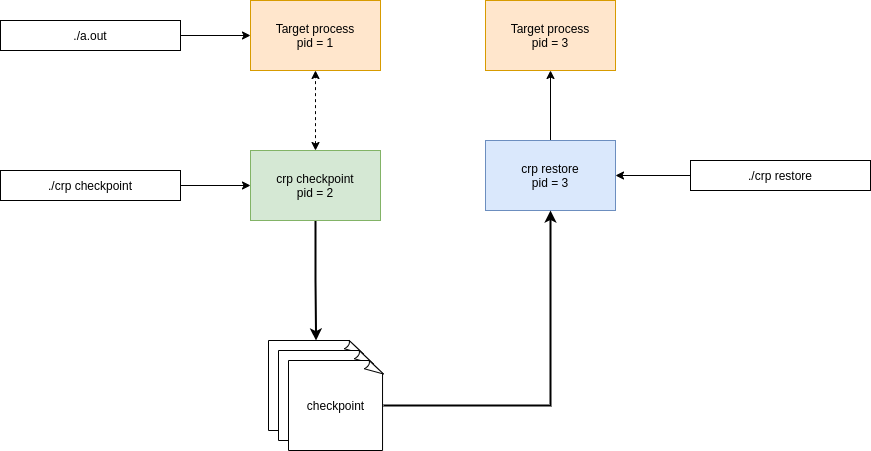
\includegraphics[width=0.6\textwidth]{crp.png}
    \caption{Checkpoint and Restore mechanism}
    \label{fig:crp}
\end{figure}

\label{sec:newproc}
\subsubsection{Restoring the Kernel State}
% Loading data and pointers restoring
As mentioned in section \ref{sec:newproc}, for updating kernel state of new process, we load the checkpointed structures (e.g. list of \verb|vm_area_struct|, \verb|mm_struct| information)

% each data struct like, mm_struct, vm_area_struct, has its own 
Major hurdle / frequent cause of faults in restoring the kernel state we found was the inherent and strong assumption in the POSIX design of kernel that every structure is available in the memory pointed by a pointer, as explained in section \ref{sec:kds}.

\subsubsection{Arch dependent register restoring/checkpointing}
% apart from copying pt_regs thread states and FS and GS registers are required depending on arch
Restoring \verb|pt_regs| is not enough for some special registers like \verb|FS|, \verb|GS|, control registers, etc. Such CPU states are stored in \verb|task_struct->thread| which is architecture dependent and requires architecture specific handling for restoring these registers. e.g. \verb|x86_fsbase_write_cpu|  has been used to restore \%fs register while for other registers it sufficies to write them to \verb|pt_regs|, which will be restored when process is scheduled.

% \subsection{Incremental checkpointing}
% % required for fault tolerence

% \subsubsection{Dirty-bit for kernel pages}
% % Naive approach for keeping track of updated kernel memory

% \subsubsection{Other approaches}
% % WHY Aurora shadowing / implementation does not help etc


\section{Source code}

\href{https://github.com/dev-chauhan/crp.git}{github.com/dev-chauhan/crp.git}
% Major problem and hurdles faced, hidden toughness of the problem

% OUR DECISION OF USING DUP MM Allowed us to find bugs in register restoring otherwise we would be stuck without knowing what is the actual problem, such small problems (like restoring FS) are big hurdles for working with linux kernel / our project
\section{Contribution}

\begin{center}
\begin{tabular}{ |c|c|c| } 
 \hline
 Dev & ideation, CPU state restore, mm restore, user facing library and base driver, kallsyms, \\
    &   reports and presentations, testing other methods for restore \\
 \hline
 Paras & ideation, VMA restore, rbtree restore, process kernel state inspection(virtual memory), \\
 & reports and presentations, testing other methods for restore \\
 \hline
 Somu &    Reading about POSIX kernel structures important for checkpoint/restore similar to Aurora\\
 \hline
\end{tabular}
\end{center}
\end{document}
